\setlength{\parskip}{0cm}
\begin{Large}
\newpage
\section{Реализация системы}
\subsection{Обзор инструментов для разработки}
Для создания игры «Монополия» был выбран язык Python, который на данный момент является передовым решением для машинного обучения, помимо этого он достаточно прост в освоении и позволяет быстро реализовать необходимые алгоритмы. Для реализации нейронной сети была выбрана библиотека Keras, которая представляет собой простой и удобный интерфейс для обучения нейронных сетей. В качестве среды разработки была выбрана PyCharm 2018.1
\subsection{Реализация интерфейса для создания ботов}
Игра «Монополия» включает в себя интерфейс для создания ботов. Для того, чтобы разработанный бот являлся полноценным актёром системы он должен реализовывать следующие методы:
\begin{enumerate}
    \item \textit{landed\_on\_unowned\_property (self, game, field)} – метод, вызываемый, когда игрок попадает на поле, не принадлежащее никому. Возвращает true – если покупка одобрена, false – покупка не одобрена
    \item \textit{property\_offered\_for\_auction (self, game, field, price)} - метод, вызываемый, когда игрок участвует в аукционе. Возвращает true – если цена устраивает, false – если цена не устраивает, и игрок хочет выйти из аукциона
    \item \textit{build\_house (self, game, field)} – метод, вызываемый, когда игроку предлагается купить дом на поле. Возвращает true – если покупка одобрена, false – покупка не одобрена
    \item \textit{sell\_house (self, game, field)} – метод, вызываемый, когда игроку предлагается продать дом на поле. Возвращает true – если продажа одобрена, false – продажа не одобрена
    \item \textit{mortgage\_property (self, game, field)} – метод, вызываемый, когда игроку предлагается заложить своё поле. Возвращает true – если залог одобрен, false – залог не одобрен
    \item \textit{redeem\_property (self, game, field)} – метод, вызываемый, когда игроку предлагается выкупить своё поле из залога. Возвращает true – если выкуп одобрен, false – выкуп не одобрен
    \item \textit{get\_out\_of\_jail (self, game)} – метод, вызываемый, когда игрок находится в тюрьме и ему предлагается выйти из тюрьмы, оплатив выкуп. Возвращает true – если выкуп одобен, false – выкуп не одобрен.
\end{enumerate}
\subsection{Реализация Q-обучения нейронной сети}
Для реализации обучения нейронной сети были сделаны несколько методов:
\begin{enumerate}
    \item \textit{select\_action (self, state)} – выбор следующего действия нейронной сети, исходя из игрового состояния
    \item \textit{record (self, state,action, reward, next\_state, done)} – запись текущих действий нейронной сети
    \item \textit{replay(self)} – функция обучения нейронной сети
\end{enumerate}
\begin{figure}[h!]
    \center{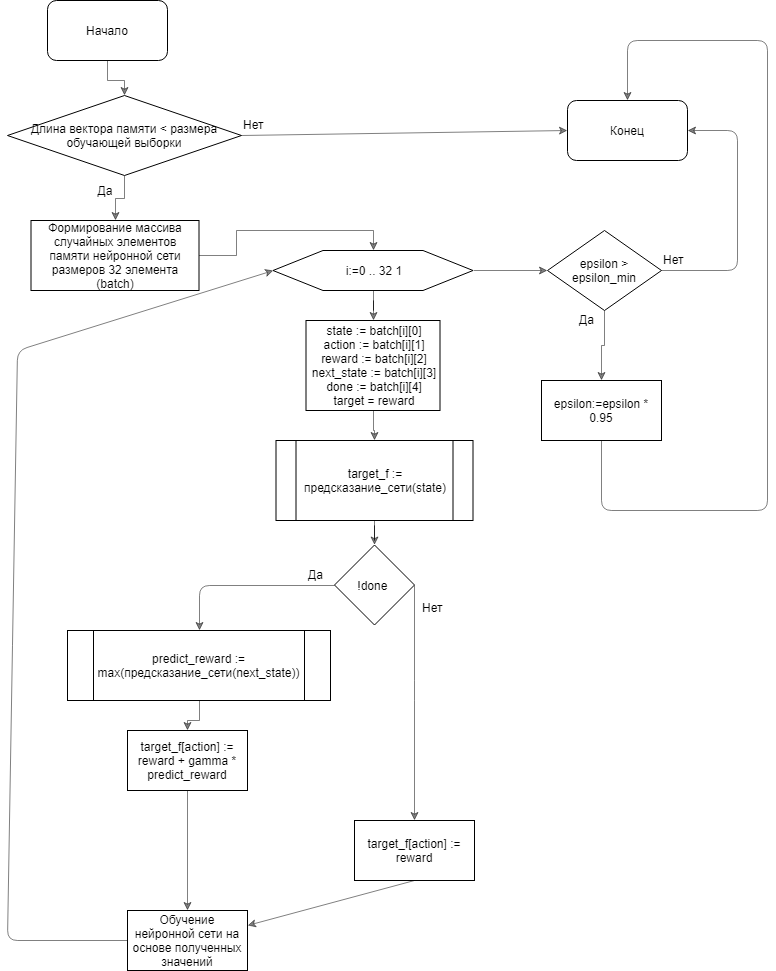
\includegraphics[scale=0.85]{bnn.png}}
    \caption{Блок-схема обучения нейронной сети}
\end{figure}
\newpage
\subsection{Реализация игровых ботов}
Для удобного обучения и тестирования нейронной сети была реализована простая логика противников. 

Первый тип противника работает по принципу случайного поведения игрока, то есть на любое предлагаемое действие он реагирует случайным образом.

Второй тип противника реализует простое поведение игрока. Основные правила, которых он придерживается:
\begin{enumerate}
    \item Согласиться с покупкой, если баланс игрока – стоимость покупки> 350
    \item Согласиться с продажей, если баланс игрока меньше 150
    \item Ничего не делать, если баланс находится в промежутке между 150 и 350.
\end{enumerate}
\subsection*{Выводы}
\addcontentsline{toc}{subsection}{Выводы}
На основе разработанной архитектуры было реализована система игра «Монополия». Выполнена реализация интерфейса для создания ботов и обучения нейронной сети.
\end{Large}